\documentclass[12pt]{article}
\usepackage{fullpage}
\usepackage[shortlabels]{enumitem}
\usepackage{amsmath}
\usepackage{amsthm}
\usepackage{graphicx}
\usepackage{amssymb}
\usepackage{enumitem}
\usepackage{tikz}

\title{250 Homework $\#$2 (Fall 2026)}
\author{Toby Hansen \footnote{Collaborated with Nobody.}}
%\author{Solution Sketches\footnote{Collaborated with Nobody.}}
\begin{document}
	\date{}
	\maketitle

	This assignment is due at 11:59 p.m. on Friday 9 October 2026, to be submitted
	on Gradescope. Late assignments (with penalty, unless excused) will be
	accepted until 11:59 p.m. on Saturday 10 October 2026, and not after. Please see
	the syllabus for more details on homework grading and late penalties.

	\medskip

	When submitting to Gradescope, please do not forget to assign pages to problems.

	\medskip

	All problems, with the exception of the first two and , originally come from the
	textbook. Some of them have been modified. In case of doubt, the version
	printed here is the one you should follow.

	\bigskip

	The instructions for this homework are the same as for HW1. Please read them
	there.

	\bigskip

	See the Canvas Homework web page for detailed instructions on how to format solutions.
	Solutions that do not follow those formatting instructions will be returned
	for rewriting and resubmission. In later assignments there will be points deducted
	for such formatting errors.

	%%%%%%%%%%%%%%%%%%%%%%%
	\newpage

	\section*{\textbf{Question 1} [10 pts]}
	{\em \small Your solution should follow the format given on pages 17-19 of the relation study guide.}

	Let $A =\{a,b,c,d,e\}$. The relation $P \subseteq A \times A$ is a
	{\bf partial order}.\\
	It is known that
	\begin{enumerate}
		\item $(a,b),(b,c),(d,e), (d,b)\in P$ and
		%\item $(a,d), (b,d),(b,e), (c,b), (c,d) \in P,$   and
		%\item  $(b,a), (e,d) \not \in P.$

		\item $(c,e), (e,b),(d,a),(b,d) \not\in P.$
	\end{enumerate}

	(i) In the table given below, label all pairs that must be in $P$ with a ``$\checkmark$''
	and all pairs that cannot be in $P$ with a ``$\times$.'' For pairs that are neither,
	leave their entry blank. We start you off by labelling the five known pairs with
	the appropriate ``$\checkmark$'' or $\times.$

	\smallskip

	For full credit, you must justify your answers. Do that by numbering your justifications
	and, next to each $\checkmark$ or $\times$ in the table, write the number of the
	justification for that entry.

	\medskip

	\[
		\small \hspace*{-.5in}
		\begin{array}{|c|c||c||c|c||c||c|c||c||c|c||c||c|c|}
			\hline
			(a,a) & \quad        &  & (b,a) &              &  & (c,a) & \quad    &  & (d,a) & \times 2     &  & (e,a) & \quad    \\
			\hline
			(a,b) & \checkmark 1 &  & (b,b) &              &  & (c,b) &          &  & (d,b) & \checkmark 1 &  & (e,b) & \times 2 \\
			\hline
			(a,c) &              &  & (b,c) & \checkmark 1 &  & (c,c) &          &  & (d,c) &              &  & (e,c) &          \\
			\hline
			(a,d) &              &  & (b,d) & \times 2     &  & (c,d) &          &  & (d,d) &              &  & (e,d) &          \\
			\hline
			(a,e) &              &  & (b,e) &              &  & (c,e) & \times 2 &  & (d,e) & \checkmark 1 &  & (e,e) &          \\
			\hline
		\end{array}
	\]

	\medskip

	\bigskip

	(ii) How many partial orders $P'$ exist such that $(a,b)$, $(b, c)$, $(d,e)$ and
	$(d, b)$ are in $P'$, and that satisfy that $(c,e)$, $(e,b)$, $(d,a)$, and $(b,
	d)$ are not in $P'$? Briefly explain how you know this.

	Draw a separate Hasse diagram for each such partial order $P'.$\\
	Note. You must draw these using the convention taught in class: an edge corresponding
	to relation $(a,b)$ must go {\em up} from $a$ to $b.$

	\bigskip

	\subsection*{\textbf{Solution:}}
	\begin{enumerate}[(i)]
		\item
			\[
				\begin{array}{|c|c||c||c|c||c||c|c||c||c|c||c||c|c|}
					\hline
					(a,a) & \checkmark3 &  & (b,a) & \times 5    &  & (c,a) & \times 5    &  & (d,a) & \times 2    &  & (e,a) & \times 6    \\
					\hline
					(a,b) & \checkmark1 &  & (b,b) & \checkmark3 &  & (c,b) & \times 5    &  & (d,b) & \checkmark1 &  & (e,b) & \times 2    \\
					\hline
					(a,c) & \checkmark4 &  & (b,c) & \checkmark1 &  & (c,c) & \checkmark3 &  & (d,c) & \checkmark4 &  & (e,c) &             \\
					\hline
					(a,d) &             &  & (b,d) & \times 2    &  & (c,d) & \times 5    &  & (d,d) & \checkmark3 &  & (e,d) & \times 5    \\
					\hline
					(a,e) &             &  & (b,e) &             &  & (c,e) & \times 2    &  & (d,e) & \checkmark1 &  & (e,e) & \checkmark3 \\
					\hline
				\end{array}
			\]
			\begin{enumerate}[1.]
				\item Its given that $(a,b),(b,c),(d,e),(d,b) \in P$

				\item Its given that $(c,e),(e,b),(d,a),(b,d) \not\in P.$

				\item Since its a partial order, it must be reflexive; therefore every identity
					pair must be present: $\forall x \in A, (x,x) \in P$; $(a,a),(b,b),(c,c
					),(d,d),(e,e) \in P$

				\item Since its a partial order, it must be transitive; therefore for any
					pairs in (1.) where the output is the same as another pair's input,
					the first pair's input must be paired with the second pair's output:
					\begin{enumerate}[a.]
						\item Since $(a,b),(b,c) \in P$; $(a,c) \in P$

						\item Since $(d,b),(b,c) \in P$; $(d,c) \in P$
					\end{enumerate}

				\item Since its a partial order, it must be antisymmetric; therefore every
					known pair from (1.) and (4.) CANNOT have a matching reverse pair (unless
					the elements are identical like identity pairs):
					$(b,a),(c,b),(e,d),(b,d),(c,a),(c,d) \not\in P$

				\item From transitivity, any pairs that would require a pair we've
					already ruled out to be present, cannot be in P; Since $(a,b) \in P$, and
					$(e,b) \not\in P$; $(e,a) \not\in P$
			\end{enumerate}

			The entries for $(a,d),(a,e),(b,e),(e,c)$ are left blank because the given
			facts cannot be used to definitively derive whether those pairs \textit{must}
			or \textit{cannot} be in P.

		\item
			% Add to preamble:

			There are 16 theoretical combinations of the four optional pairs ($2^{4}$),
			but only \textbf{10} of those 16 are actually possible with the given conditions.

			\textbf{P01: } $(a,d),(a,e),(b,e),(e,c) \not\in P$ \\
			This is the minimal partial order with none of the four optional pairs
			included. Transitivity provides the $(a,c)$ and $(d,c)$ pairs in the graph.
			\begin{center}
				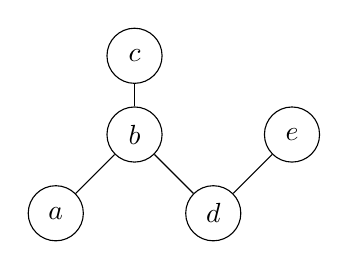
\begin{tikzpicture}[every node/.style={circle,draw,minimum size=7mm}]
					\node (a) at (0,0) {$a$};
					\node (b) at (1,1) {$b$};
					\node (c) at (1,2) {$c$};
					\node (d) at (2,0) {$d$};
					\node (e) at (3,1) {$e$};
					\draw (a) -- (b);
					\draw (d) -- (b);
					\draw (b) -- (c);
					\draw (d) -- (e);
				\end{tikzpicture}
			\end{center}

			\textbf{P02: } $(a,d),(a,e),(b,e) \not\in P$ and $(e,c) \in P$ \\
			This partial order includes 1 of the four optional pairs $(e,c)$. None of the
			other optional pairs need to be included through transitivity.
			Transitivity provides the $(a,c),(d,c)$ pairs in the graph.
			\begin{center}
				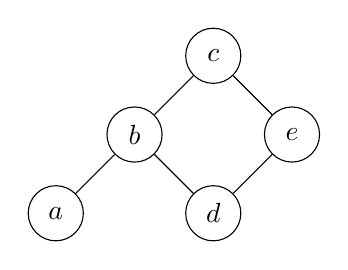
\begin{tikzpicture}[every node/.style={circle,draw,minimum size=7mm}]
					\node (a) at (0,0) {$a$};
					\node (d) at (2,0) {$d$};
					\node (b) at (1,1) {$b$};
					\node (e) at (3,1) {$e$};
					\node (c) at (2,2) {$c$};
					\draw (a) -- (b);
					\draw (d) -- (b);
					\draw (b) -- (c);
					\draw (d) -- (e);
					\draw (e) -- (c);
				\end{tikzpicture}
			\end{center}

			\textbf{P03: } $(a,d),(e,c),(b,e) \not\in P$ and $(a,e) \in P$ \\
			This partial order includes 1 of the four optional pairs $(a,e)$. None of
			the other optional pairs need to be included through transitivity. Transitivity
			provides the $(a,c),(d,c)$ pairs in the graph.
			\begin{center}
				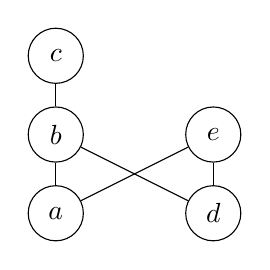
\begin{tikzpicture}[every node/.style={circle,draw,minimum size=7mm}]
					\node (a) at (0,0) {$a$};
					\node (b) at (0,1) {$b$};
					\node (c) at (0,2) {$c$};
					\node (d) at (2,0) {$d$};
					\node (e) at (2,1) {$e$};
					\draw (a) -- (b);
					\draw (a) -- (e);
					\draw (d) -- (b);
					\draw (d) -- (e);
					\draw (b) -- (c);
				\end{tikzpicture}
			\end{center}

			\textbf{P04: } $(a,d),(b,e) \not\in P$ and $(a,e),(e,c) \in P$ \\
			This partial order includes the 2 optional pairs $(a,e),(e,c)$ that can be
			flipped independently of the other optional pairs (as seen in P03 and P02).
			Transitivity provides the $(a,c),(d,c)$ pairs in the graph.
			\begin{center}
				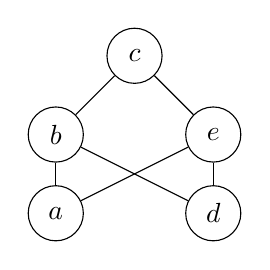
\begin{tikzpicture}[every node/.style={circle,draw,minimum size=7mm}]
					\node (a) at (0,0) {$a$};
					\node (b) at (0,1) {$b$};
					\node (c) at (1,2) {$c$};
					\node (d) at (2,0) {$d$};
					\node (e) at (2,1) {$e$};
					\draw (a) -- (b);
					\draw (a) -- (e);
					\draw (d) -- (b);
					\draw (d) -- (e);
					\draw (b) -- (c);
					\draw (e) -- (c);
				\end{tikzpicture}
			\end{center}

			\textbf{P05: } $(b,e),(e,c) \not\in P$ and $(a,d),(a,e) \in P$ \\
			Including $(a,d)$ REQUIRES including $(a,e)$ through transitivity, since $(
			d,e)$ exists in all variations of P. Transitivity provides the
			$(a,c),(a,b),(a,e),(d,c)$ pairs in the graph.
			\begin{center}
				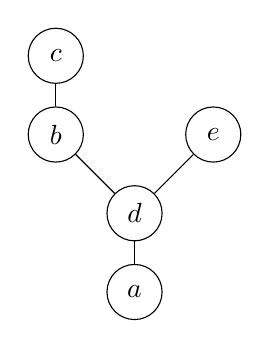
\begin{tikzpicture}[every node/.style={circle,draw,minimum size=7mm}]
					\node (a) at (1,0) {$a$};
					\node (b) at (0,2) {$b$};
					\node (c) at (0,3) {$c$};
					\node (d) at (1,1) {$d$};
					\node (e) at (2,2) {$e$};
					\draw (a) -- (d);
					\draw (d) -- (b);
					\draw (d) -- (e);
					\draw (b) -- (c);
				\end{tikzpicture}
			\end{center}

			\textbf{P06: } $(b,e) \not\in P$ and $(a,d),(a,e),(e,c) \in P$ \\
			This is the same as P04, just with the independent $(e,c)$ included as
			well. Transitivity provides the $(a,c),(a,b),(a,e),(d,c)$ pairs in the graph.
			\begin{center}
				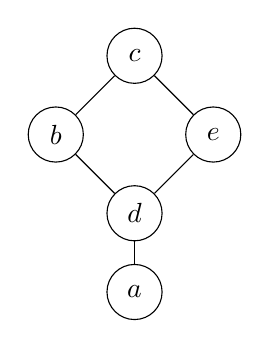
\begin{tikzpicture}[every node/.style={circle,draw,minimum size=7mm}]
					\node (a) at (1,0) {$a$};
					\node (b) at (0,2) {$b$};
					\node (c) at (1,3) {$c$};
					\node (d) at (1,1) {$d$};
					\node (e) at (2,2) {$e$};
					\draw (a) -- (d);
					\draw (d) -- (b);
					\draw (d) -- (e);
					\draw (b) -- (c);
					\draw (e) -- (c);
				\end{tikzpicture}
			\end{center}

			\textbf{P07: } $(a,d),(e,c) \not\in P$ and $(b,e),(a,e) \in P$ \\
			Including $(b,e)$ REQUIRES including $(a,e)$ through transitivity, since $(
			a,b)$ exists in all variations of P. Transitivity provides the
			$(a,c),(d,e),(a,e),(d,c)$ pairs in the graph.
			\begin{center}
				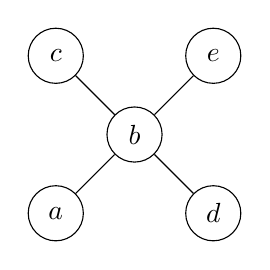
\begin{tikzpicture}[every node/.style={circle,draw,minimum size=7mm}]
					\node (a) at (0,0) {$a$};
					\node (d) at (2,0) {$d$};
					\node (b) at (1,1) {$b$};
					\node (e) at (2,2) {$e$};
					\node (c) at (0,2) {$c$};
					\draw (a) -- (b);
					\draw (b) -- (c);
					\draw (d) -- (b);
					\draw (b) -- (e);
				\end{tikzpicture}
			\end{center}

			\textbf{P08: } $(a,d) \not\in P$ and $(b,e),(a,e),(e,c) \in P$ \\
			This is the same as P06, just with the independent $(e,c)$ included as
			well. Transitivity provides the $(a,c),(d,e),(a,e),(d,c),(b,c)$ pairs in the
			graph.
			\begin{center}
				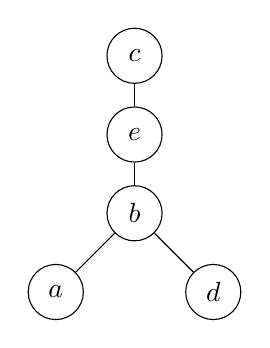
\begin{tikzpicture}[every node/.style={circle,draw,minimum size=7mm}]
					\node (a) at (0,0) {$a$};
					\node (d) at (2,0) {$d$};
					\node (b) at (1,1) {$b$};
					\node (e) at (1,2) {$e$};
					\node (c) at (1,3) {$c$};
					\draw (a) -- (b);
					\draw (e) -- (c);
					\draw (d) -- (b);
					\draw (b) -- (e);
				\end{tikzpicture}
			\end{center}

			\textbf{P09: } $(e,c) \not\in P$ and $(a,d),(b,e),(a,e) \in P$ \\
			This is the same as P06, but since $(a,d)$ ALSO requires including $(a,e)$,
			we can make a version with all 3. Transitivity provides the
			$(a,c),(a,b),(a,e),(d,c),(d,e)$ pairs in the graph.
			\begin{center}
				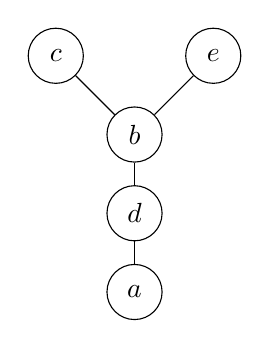
\begin{tikzpicture}[every node/.style={circle,draw,minimum size=7mm}]
					\node (a) at (1,0) {$a$};
					\node (d) at (1,1) {$d$};
					\node (b) at (1,2) {$b$};
					\node (e) at (2,3) {$e$};
					\node (c) at (0,3) {$c$};
					\draw (a) -- (d);
					\draw (b) -- (c);
					\draw (d) -- (b);
					\draw (b) -- (e);
				\end{tikzpicture}
			\end{center}

			\textbf{P10: } $(e,c),(a,d),(b,e),(a,e) \in P$ \\
			This is the same as P08, just with the independent $(e,c)$ included as
			well. Transitivity provides the $(a,c),(a,b),(a,e),(d,c),(d,e),(d,c)$ pairs
			in the graph.
			\begin{center}
				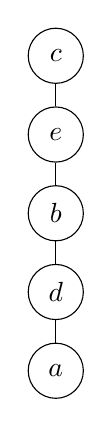
\begin{tikzpicture}[every node/.style={circle,draw,minimum size=7mm}]
					\node (a) at (0,0) {$a$};
					\node (d) at (0,1) {$d$};
					\node (b) at (0,2) {$b$};
					\node (e) at (0,3) {$e$};
					\node (c) at (0,4) {$c$};
					\draw (a) -- (d);
					\draw (d) -- (b);
					\draw (b) -- (e);
					\draw (e) -- (c);
				\end{tikzpicture}
			\end{center}
	\end{enumerate}

	%%%%%%%%%%%%%%%%%%%%

	\newpage

	\section*{\textbf{Question 2} [10 pts]}
	{\em \small Your solution should follow the format given on pages 20-23 of the relation study guide.}

	\medskip

	Let $A =\{a,b,c,d,e,f,g\}$. The relation $Q \subseteq A \times A$ is an {\bf equivalence relation}.\\
	It is known that
	\begin{enumerate}
		\item $(a,b), (c,d),(e,f)\in Q,$ and

		\item $(c,f), (g,e)\not \in Q.$
	\end{enumerate}

	\medskip

	\par
	\noindent
	{(i)} In the table given below, label all pairs that must be in $Q$ with a ``$\checkmark$''
	and all pairs that cannot be in $Q$ with a ``$\times$.'' For pairs that are neither,
	leave their entry blank. We start you off by labelling the five known pairs with
	the appropriate ``$\checkmark$'' or $\times.$

	\smallskip

	For full credit, you must justify your answers. Do that by numbering your justifications
	and, next to each $\checkmark$ or $\times$ in the table, write the number of the
	justification for that entry.

	\[
		\small \hspace*{-.5in}
		\begin{array}{|c|c||c||c|c||c||c|c||c||c|c||c||c|c||c|| c|c|| c|| c| c|}
			\hline
			(a,a) & \quad        &  & (b,a) & \quad &  & (c,a) & \quad        &  & (d,a) & \quad &  & (e,a) & \quad        &  & (f,a) & \quad &  & (g,a) & \quad    \\
			\hline
			(a,b) & \checkmark 1 &  & (b,b) &       &  & (c,b) &              &  & (d,b) &       &  & (e,b) &              &  & (f,b) &       &  & (g,b) &          \\
			\hline
			(a,c) & \quad        &  & (b,c) & \quad &  & (c,c) & \quad        &  & (d,c) & \quad &  & (e,c) & \quad        &  & (f,c) & \quad &  & (g,c) & \quad    \\
			\hline
			(a,d) &              &  & (b,d) &       &  & (c,d) & \checkmark 1 &  & (d,d) &       &  & (e,d) &              &  & (f,d) &       &  & (g,d) &          \\
			\hline
			(a,e) &              &  & (b,e) &       &  & (c,e) &              &  & (d,e) &       &  & (e,e) &              &  & (f,e) &       &  & (g,e) & \times 2 \\
			\hline
			(a,f) &              &  & (b,f) &       &  & (c,f) & \times 2     &  & (d,f) &       &  & (e,f) & \checkmark 1 &  & (f,f) &       &  & (g,f) &          \\
			\hline
			(a,g) &              &  & (b,g) &       &  & (c,g) &              &  & (d,g) &       &  & (e,g) &              &  & (f,g) &       &  & (g,g) &          \\
			\hline
		\end{array}
	\]
	\bigskip

	\bigskip

	\par
	\noindent
	{(ii)} (a) How many equivalence relations $Q'$ exist that satisfy $(a,b), (c,d)
	,(e,f)\in Q',$ and $(c,f), (g,e) \not \in Q'?$

	%$(a,b), (c,b),(d,b), (e,f) \in Q',$   and $(e,b) \not \in Q'.$
	%Briefly explain how you know this.

	(b) Also, write down, in partition format, all of the equivalence relations
	that satisfy the 5 known pairs. It is not necessary to show how you derived them.

	When writing down a partition, each of the subsets should be written in
	alphabetical order with each set being written in alphabetical order and the
	order of the sets being the alphabetical ordering of their `first' element. For
	example, the equivalence relation that has $g,c,e$ together, $d,b$ together and
	$a,f$ together should be written as $\Bigl\{ \{a,f\}, \, \{b,d\},\, \{c,e,g\}\Bigr
	\}.$

	\subsection*{\textbf{Solution:}}
	\begin{enumerate}[(i)]
		\item
			\[
				\scriptsize
				\begin{array}{|c|c||c||c|c||c||c|c||c||c|c||c||c|c||c||c|c||c||c|c|}
					\hline
					(a,a) & \checkmark3 &  & (b,a) & \checkmark5 &  & (c,a) &             &  & (d,a) &             &  & (e,a) &             &  & (f,a) &             &  & (g,a) &             \\
					\hline
					(a,b) & \checkmark1 &  & (b,b) & \checkmark3 &  & (c,b) &             &  & (d,b) &             &  & (e,b) &             &  & (f,b) &             &  & (g,b) &             \\
					\hline
					(a,c) &             &  & (b,c) &             &  & (c,c) & \checkmark3 &  & (d,c) & \checkmark5 &  & (e,c) & \times 5    &  & (f,c) & \times 5    &  & (g,c) &             \\
					\hline
					(a,d) &             &  & (b,d) &             &  & (c,d) & \checkmark1 &  & (d,d) & \checkmark3 &  & (e,d) & \times 5    &  & (f,d) & \times 5    &  & (g,d) &             \\
					\hline
					(a,e) &             &  & (b,e) &             &  & (c,e) & \times 4    &  & (d,e) & \times 4    &  & (e,e) & \checkmark3 &  & (f,e) & \checkmark5 &  & (g,e) & \times 2    \\
					\hline
					(a,f) &             &  & (b,f) &             &  & (c,f) & \times 2    &  & (d,f) & \times 4    &  & (e,f) & \checkmark1 &  & (f,f) & \checkmark3 &  & (g,f) & \times 6    \\
					\hline
					(a,g) &             &  & (b,g) &             &  & (c,g) &             &  & (d,g) &             &  & (e,g) & \times 5    &  & (f,g) & \times 6    &  & (g,g) & \checkmark3 \\
					\hline
				\end{array}
			\]
			\begin{enumerate}[1.]
				\item Its given that $(a,b),(c,d),(e,f) \in Q$

				\item Its given that $(c,f),(g,e) \not\in Q$

				\item Since its an equivalence relation, it must be reflexive; therefore
					every identity pair must be present: $\forall x \in A, (x,x) \in Q$; $(
					a,a),(b,b),(c,c),(d,d),(e,e),(f,f),(g,g) \in Q$

				\item Since its an equivalence relation, it must be transitive; therefore
					any pairs that would require a pair we've already excluded to be included,
					cannot be in Q since they imply a pair that CANNOT be included:
					\begin{enumerate}[-]
						\item Since $(c,d) \in Q$, and $(c,f) \not\in Q$; $(d,f) \not\in Q$

						\item Since $(e,f) \in Q$, and $(c,f) \not\in Q$; $(c,e) \not\in Q$

						\item Since $(c,d),(e,f) \in Q$, and $(c,f) \not\in Q$; $(d,e) \not\in
							Q$
					\end{enumerate}

				\item Since its an equivalence relation, it must be symmetric; therefore
					every known pair from (1.) MUST have a matching reverse pair included,
					and every known pair from (2.) and (4.) CANNOT have a matching reverse
					pairs included: $(b,a),(d,c),(f,e) \in Q$, and
					$(f,c),(e,g),(f,d),(e,c),(e,d) \not\in Q$

				\item Just like in (4.), because of transitivity, since $(e,f) \in Q$,
					and $(e,g) \not\in Q$; $(f,g) \not\in Q$; Also, just like in (5.),
					because of symmetry, $(g,f) \not\in Q$
			\end{enumerate}
			The remaining entries are left blank because the given facts cannot be used
			to definitively derive whether those pairs \textit{must} or \textit{cannot}
			be in Q.

		\item
			\begin{enumerate}[(a)]
				\item From part (i), the initial equivalence classes are
					$\{a,b\},\{c,d\},\{e,f\},\{g\}$.

					Since $(c,f)$ is excluded, the classes $\{c,d\}$ and $\{e,f\}$ cannot be
					merged. Similarly, since $(g,e)$ is excluded, the classes $\{e,f\}$
					and $\{g\}$ cannot be merged. With the given conditions, exactly
					\textbf{7} possible combinations exist.

				\item
					\begin{enumerate}[1.]
						\item $\Bigl\{ \{a,b\},\{c,d\},\{e,f\},\{g\} \Bigr\}$ (The initial
							relation)

						\item $\Bigl\{ \{a,b,c,d\},\{e,f\},\{g\} \Bigr\}$ (Merge a,b and c,d)

						\item $\Bigl\{ \{a,b,e,f\},\{c,d\},\{g\} \Bigr\}$ (Merge a,b and e,f)

						\item $\Bigl\{ \{a,b,g\},\{c,d\},\{e,f\} \Bigr\}$ (Merge a,b and g)

						\item $\Bigl\{ \{a,b\},\{c,d,g\},\{e,f\} \Bigr\}$ (Merge c,d and g)

						\item $\Bigl\{ \{a,b,c,d,g\},\{e,f\} \Bigr\}$ (Merge a,b and c,d and
							g)

						\item $\Bigl\{ \{a,b,e,f\},\{c,d,g\} \Bigr\}$ (Merge a,b and e,f; Merge
							c,d and g)
					\end{enumerate}
			\end{enumerate}
	\end{enumerate}

	%%%%%%%%%%%%%%%%%%
	\newpage

	\section*{\textbf{Question 3. P2.1.7} [10 pts]}
	Let $X$ be a set of at least two people. We will ask each person in $X$ to write
	down the name of a person in $X$ other than themself. Let $R$ be the relation
	$\{\langle a, b\rangle$ : $a$’s chosen name is $b\}$. Suppose we start with a
	given person $a$, move to the person that $a$ wrote down, then to the person
	that they wrote down, and so forth until we reach a given person $b$. Let $S$
	be the relation
	\[
		S =\{\langle a, b\rangle: \mbox{Starting from $a$, we eventually reach $b$ by
		this process}\}.
	\]
	\begin{enumerate}[(a)]
		\item If from $a$, we reach $a$ again before finding $b$, explain why we will
			never reach $b$.

		\item If $\langle a, b\rangle$ is not in $S$, when can we give up on the
			process, i.e., be sure that $\langle a, b\rangle$ is not in $S.$

		\item If $\langle a, b\rangle$ is not in $S$, will we definitely reach $a$. i.e.,
			is $\langle a, a\rangle$ in $S?$ If the answer is yes, prove it. If the answer
			is no, give a counterexample in which $\langle a, b\rangle \not\in S$ but
			$\langle a, a\rangle \not\in S.$
	\end{enumerate}

	\subsection*{\textbf{Solution:}} %MJG
	\begin{enumerate}[(a)]
		\item If from \textit{a}, we reach \textit{a} again before finding \textit{b},
			we will never reach \textit{b}. This is because if we circle back to
			\textit{a}, it must be a cycle/loop since each person only writes down a
			single name (each input only has 1 output); and since a loop repeats infinitely,
			we would never get the chance to reach \textit{b}, which lies OUTSIDE the
			loop.

		\item We can give up on the process and conclude that $\langle a,b \rangle \not
			\in S$ if and ONLY if, we see a person's name more than once before
			finding \textit{b}. This is because seeing a person's name more than once
			signifies an infinite loop, and if we hadn't found \textit{b} by then, it'll
			never come up in the infinite loop that is made up of people we've already
			checked.

		\item If $\langle a, b\rangle$ is not in $S$, that does NOT necessarily mean
			that $\langle a, a\rangle$ is in $S$. Just because an infinite loop is reached,
			does not mean that it has to include all the way back as far as \textit{a};
			for example, if \textit{a} wrote down \textit{x}, \textit{x} write down \textit{y},
			and \textit{y} wrote down \textit{x}, then even though you started with
			\textit{a} and got caught in an infinite loop, the loop is just going back
			and forth between \textit{x} and \textit{y}.
	\end{enumerate}

	%%%%%%%%%%%%%%%%%%
	\newpage

	\section*{\textbf{Question 4. P2.3.3} [10 pts]}
	Let $A$ and $B$ be two types such that $A$ is a proper subset of $B$ ($A \subset
	B$, i.e., so that $B$ contains all the elements of $A$ plus at least one other
	element). Let $P$ be a unary predicate on $A$, and let $Q$ be a unary predicate
	on $B$. Suppose that $\forall a: \forall b : P(a) \rightarrow Q(b)$ is true.

	Which of the following four statements is guaranteed to be true? For each statement,
	explain why it is always true or give an example where it is false. (Hint: Consider
	the case where $A$ is empty.)
	\begin{enumerate}[(a)]
		\item ($\forall a : P(a)$) $\rightarrow$ ($\forall b : Q(b)$)

		\item ($\forall b : Q(b)$) $\rightarrow$ ($\forall a : P(a)$)

		\item ($\exists a : P(a)$) $\rightarrow$ ($\exists b : Q(b)$)

		\item ($\exists b : Q(b)$) $\rightarrow$ ($\exists a : P(a)$)
	\end{enumerate}

	\subsection*{\textbf{Solution:}}
	In English, the given condition that is always true is: For every element of A
	and B, if the element of A satisfies P, then the element of B must satisfy Q
	\begin{enumerate}[(a)]
		\item FALSE\\
			In English, if every element of A satisfies P, then every element of B
			satisfies Q.\\
			Although it sounds nearly identical to the given condition, consider the empty
			set for A; P will always evaluate to TRUE since there are no
			counterexamples, meanwhile if even 1 value of B (which must have at least
			1 value in a addition to the empty set) doesn't satisfy Q, then the
			implication is false. For example: P(x) is defined as "\textit{x is not
			equal to 67}", Q(x) is defined as "\textit{x is equal to 2}", A is the
			empty set, B is the set {1};

		\item FALSE\\
			In English, if every element of B satisfies Q, then every element of A
			satisfies P.\\
			According to the given condition, whether or not elements of B satisfy Q has
			no bearing on whether or not elements of A satisfy P. For example: P(x) is
			defined as "\textit{x is less than 1}", Q(x) is defined as \textit{x is
			greater than 5}, A is the set {6}, B is the set {6,7}.

		\item TRUE\\
			In English, if at least one element of A satisfies P, then at least one
			element of B satisfies Q.\\
			Since there needs to be at least one element in A for this proposition, the
			empty set trick won't work this time, if we do set A to the empty set it
			will just be false since there isn't at least one element. With the given condition,
			it is impossible for an element of A to satisfy P without an element of B
			satisfying Q, therefore this statement is guaranteed to be true.

		\item FALSE\\
			In English, if at least one element of B satisfies Q, then at least one
			element of A satisfies P.\\
			According to the given condition, whether or not elements of B satisfy Q has
			no bearing on whether or not elements of A satisfy P. For example: P(x) is
			defined as "\textit{x is less than 1}", Q(x) is defined as \textit{x is
			equal to 7}, A is the set {6}, B is the set {6,7}.
	\end{enumerate}

	%%%%%%%%%%%%%%%%%%
	\newpage

	\section*{\textbf{Question 5. Modified from P2.3.8} [10 pts]}
	Let $X$ be a set and $R(x)$ a unary predicate on $X$.

	\begin{enumerate}[(a)]
		\item Write a quantified statement that says “there is exactly one element $x$
			in $X$ such that $R(x)$ is true”.

		\item Write a quantified statement that says “there are exactly two elements
			$x$ in $X$ such that $R(x)$ is true”.

		\item Write a quantified statement that says “there are at least three elements
			$x$ in $X$ with $R(x)$ true, and at least three with $R(x)$ false”

			{\em \small Note: (a) is so common that there is shorthand macro for writing it. ``\, $\exists! x: R(x)$'' denotes that there is a unique $x \in X$ satisfying $R(x),$ which is what (a) is stating. This problem is asking you how to write this from scratch.

			Your statements may use the binary relations $x = y$ and $x \neq y).$}
	\end{enumerate}

	\subsection*{\textbf{Solution:}}
	\begin{enumerate}[(a)]
		\item $\exists a \in X: (R(a) \land (\forall c \in X: (c\not=a) \rightarrow \lnot
			R(c)))$

		\item $\exists a,b \in X: (R(a) \land R(b) \land (a\not=b) \land (\forall c \in
			X: (c\not=a \land c\not=b) \rightarrow \lnot R(c)))$

		\item $\exists a,b,c,d,e,f \in X: (R(a) \land R(b) \land R(c) \land \lnot R(d
			) \land \lnot R(e) \land \lnot R(f) \land (a\not=b) \land (a\not=c) \land (
			b\not=c) \land (d\not=e) \land (d\not=f) \land (e\not=f))$
	\end{enumerate}

	% %%%%%%%%%%%%%%%%%%
	\newpage
	\section*{\textbf{Question 6. P2.6.10} [10 pts]}
	One day, a set of five dogs met after their morning walks to compare their observations
	of birds. The set $D$ of dogs consisted exactly of Arly ($a$), Cardie ($c$),
	Duncan ($d$), Mia ($m$), and Whistle ($w$).

	The set $S$ of bird species in question consisted exactly of Bluebird ($B$), Crow
	($C$), Heron ($H$), Mallard ($M$), and Woodpecker ($W$).

	The predicate $R(x, y)$ means “dog $x$ observed a bird of species $y$”.

	(a) Translate the following statements into symbolic language.
	\begin{enumerate}[I.]
		\item There was a species that was observed by all the dogs.

		\item Arly observed a Crow and no other species.

		\item Every dog other than Arly observed at least two different species.

		\item Each dog, other than Arly and Cardie, observed all the species that Cardie
			observed and at least one that Cardie did not. (Note: Different dogs may
			have observed different species that Cardie did not.)

		\item Duncan was the one and only dog to observe a Woodpecker, and Whistle
			was the one and only dog to observe a Bluebird.
	\end{enumerate}
	(b) Use statements (I)-(V) to prove that some dog observed a Heron, i.e., $\exists
	x: R(x,H).$

	Your proof should provide all steps. In particular, it should explicitly state
	when Instantiation, Specialization, etc are used.

	\subsection*{\textbf{Solution:}}
	\begin{enumerate}[(a)]
		\item
			\begin{enumerate}[I.]
				\item $\exists y \in S: \forall x \in D: R(x,y)$

				\item $R(a,C) \land\lnot R(a,B) \land\lnot R(a,H) \land\lnot R(a,M) \land
					\lnot R(a,W)$

				\item $\forall x \in D: (x\not=a \rightarrow (\exists y,z \in S: (y\not=z
					) \land R(x,y) \land R(x,z)))$

				\item $\forall x \in D: (x\not=a \land x\not=c) \rightarrow (\exists y \in
					S: (R(x,y) \land \lnot R(c,y)) \land \forall z \in S: (R(c,z) \rightarrow
					R(x, z)))$

				\item $R(d,W) \land R(w,B) \land (\forall x \in D: (x\not=d \rightarrow \lnot
					R(x,W)) \land (x\not=w \rightarrow \lnot R(x,B)))$
			\end{enumerate}

		\item We want to prove that $\exists x \in D: R(x,H)$.

			\begin{enumerate}[1.]
				\item Statement (I) says theres a species that every dog observed. By
					instantiation, this species can be $s$. $\forall x \in D: R(x,s)$

				\item Statement (II) says that Arly observed only a Crow, and since
					theres a species that EVERY dog observed, the species MUST be Crow, as
					its the ONLY one Arly observed. By substitution, $s=C$ and
					$\forall x \in D: R(x,C)$

				\item Statement (V) says that Duncan was the only dog to observe Woodpecker,
					and Whistle was the only dog to observe Bluebird. Statement (III) says
					that every dog other than Arly observed at least two different Species.
					Cardie is not Arly, Duncan, or Whistle, so Cardie MUST have seen either
					Heron or Mallard (or both) in addition to Crow (which everyone has
					seen, given by step 2): $R(c,H) \lor R(c,M)$

				\item
					\begin{enumerate}[(i)]
						\item Case 1 from step 3 supposes $R(c,H)$; Since $c \in D$, generalization
							gives $\exists x \in D: R(x,H)$

						\item Case 2 from step 3 supposes both $R(c,H) \land R(c,M)$; Since
							$c \in D$, generalization gives $\exists x \in D: R(x,H)$

						\item Case 3 from step 3 supposes $R(c,M) \land \lnot R(c,H)$. By
							statement (IV), every dog other than Arly and Cardie observed at least
							one species that Cardie did not (Heron, Bluebird, and Woodpecker).
							Duncan could have just observed a Woodpecker in addition, and Whistle
							could've just observed a Bluebird in addition; but that still
							leaves Mia, who couldn't have observed a Bluebird or Woodpecker,
							since Whistle and Duncan respectively were the ONLY dogs to
							observe them; therefore the only remaining species Mia could have observed
							in addition to the specias Cardie observed is Heron: thus $R(m,H)$
							must be true, and since $m \in D$, generalization gives
							$\exists x \in D: R(x,H)$
					\end{enumerate}

				\item Proof by cases proved that in all 3 cases,
					$\exists x \in D: R(x,H)$ is true; therefore $\exists x \in D: R(x,H)$
			\end{enumerate}
	\end{enumerate}
	\newpage

	%%%%%%%%%%%%%%%%%%
	\newpage

	\section*{\textbf{Question 7. P2.9.5} [10 pts]}
	{\em \small Note: Be aware that, in the textbook, this problem spans two pages. Also, the solution to this one is long.}

	Let $A = \{v, w\}$ and $B = \{x, y, z\}$ be sets of characters.

	\begin{enumerate}[(a)]
		\item List all the possible functions from $A$ to $B$. Determine which are
			injections.

		\item List all the possible functions from $B$ to $A$. Determine which are
			surjections.

		\item How many possible functions are there from $A$ to $A$? How many can be
			expressed as $g \circ f$, where $f$ is a function from $A$ to $B$ and $g$ is
			a function from $B$ to $A$?

		\item How many possible functions are there from $B$ to $B$? How many can be
			expressed as $f \circ g$, where $g$ and $f$ are functions as above?
	\end{enumerate}

	\subsection*{\textbf{Solution:}}
	\begin{enumerate}[(a)]
		\item A function is an injection when the distinct inputs have distinct outputs
			(when $f(v)\not= f(w)$).
			\begin{enumerate}[1.]
				\item $\{(v,x),(w,x)\}$ -- NOT injection

				\item $\{(v,x),(w,y)\}$ -- injection

				\item $\{(v,x),(w,z)\}$ -- injection

				\item $\{(v,y),(w,x)\}$ -- injection

				\item $\{(v,y),(w,y)\}$ -- NOT injection

				\item $\{(v,y),(w,z)\}$ -- injection

				\item $\{(v,z),(w,x)\}$ -- injection

				\item $\{(v,z),(w,y)\}$ -- injection

				\item $\{(v,z),(w,z)\}$ -- NOT injection
			\end{enumerate}

		\item A function is a surjection if every element of the set the function is
			being applied \textit{TO} is present in the outputs (both $v$ and $w$ appear
			as outputs).
			\begin{enumerate}[1.]
				\item $\{(x,v),(y,v),(z,v)\}$ -- NOT surjection

				\item $\{(x,v),(y,v),(z,w)\}$ -- surjection

				\item $\{(x,v),(y,w),(z,v)\}$ -- surjection

				\item $\{(x,v),(y,w),(z,w)\}$ -- surjection

				\item $\{(x,w),(y,v),(z,v)\}$ -- surjection

				\item $\{(x,w),(y,v),(z,w)\}$ -- surjection

				\item $\{(x,w),(y,w),(z,v)\}$ -- surjection

				\item $\{(x,w),(y,w),(z,w)\}$ -- NOT surjection
			\end{enumerate}

		\item There are 4 possible functions from $A$ to $A$ ($2^{2}$), and all 4
			can be expressed as $g \circ f$, where $f$ is a function from $A$ to $B$ and
			$g$ is a function from $B$ to $A$; this is because $f$ and $g$ can both
			produce 2 outputs, exactly what ALL $A$ to $A$ functions need.

		\item There are 27 possible functions from $B$ to $B$ ($3^{3}$), but only 21
			can be expressed as $f \circ g$, where $f$ is a function from $A$ to $B$ and
			$g$ is a function from $B$ to $A$; this is because $f$ and $g$ can both
			only produce 2 outputs, so you have to exclude the 6 functions from $B$ to
			$B$ that have 3 distinct outputs.
	\end{enumerate}

	%%%%%%%%%%%%%%%%%%
	\newpage

	\section*{\textbf{Question 8. P3.1.4} [10 pts]}
	The $\textbf{least common multiple}$ of two naturals $x$ and $y$ is the
	$smalle st$ natural that both $x$ and $y$ divide. For example, $lcm$(8, 12) =
	24 because 8 and 12 each divide 24, and there is no smaller natural that both 8
	and 12 divide.
	\begin{enumerate}[(a)]
		\item Find the least common multiple of 60 and 339. \\
			Write it out as a number and not, e.g., as its prime factorization.

		\item Find the least common multiple of $2^{3}\cdot 3^{2}\cdot 5^{4}$ and $2^{2}
			\cdot 3^{4}\cdot 5^{3}$. \\
			Write it out as a number and not, e.g., as its prime factorization

		\item Describe a general method to find the least common multiple of two naturals,
			given their factorization into primes (and assuming that the factorization
			exists and is unique). Write your solution in terms of $p_{i}(m)$ and $p_{i}
			(n)$ as described below.

			{\em Notation:} Let $p_{i}$ be the $i$'th prime. For natural $m,$ let
			$p_{i}(m)$ be the exponent of $p_{i}$ in the prime factorization of $m,$ i.e.,
			the largest power in $p_{i}$ that divides $m.$ So
			$m= \prod_{i=1}^{\infty}p_{i}^{p_i(m)}.$ Example: $p_{1}=2,$ $p_{2}=3$ and
			$p_{3}=5.$ Since $20= 2^{2}\cdot 5^{1},$ $p_{1}(20)=2,$ $p_{2}(20)=0,$ $p_{3}
			(20)=1$ and, $\forall i > 3,$ $p_{i}(20)=0.$
	\end{enumerate}

	\subsection*{\textbf{Solution:}}
	\begin{enumerate}[(a)]
		\item $60=2^{2}\cdot3\cdot5$ and $339=3\cdot113$\\
			Therefore, $2^{2}\cdot3\cdot5\cdot113=6780$

		\item $2^{3}\cdot3^{4}\cdot5^{4}=405000$

		\item $lcm(m,n)=\prod_{i=1}^{\infty}p_{i}^{\max(p_i(m),p_i(n))}$ \\
			For each prime, choose the larger exponent, then multiply the prime powers
			together.
	\end{enumerate}

	\newpage

	\section*{\textbf{Extra Credit. P2.1.10 in the book.} [10 pts]}
	Let $C$ be a set of $n$ candidates and $J$ be a set of $n$ jobs. Define the
	relation $Q$ to be
	\[
		Q = \{\langle c, j\rangle \,:\, \mbox{candidate $c$ is qualified for job $j$}
		\}
	\]
	Define the relation $A$ to be
	\[
		A = \{\langle c, j\rangle \,:\, \mbox{candidate $c$ is assigned to job $j$}\}
		.
	\]
	\begin{enumerate}[(a)]
		\item We say that candidate $c$ is “possible” for job $j$ if they are qualified
			for $j$, they are not assigned to any other job, and no one else is assigned
			to $j$. Informally describe how you would determine, given boolean arrays for
			the relations $Q$ and $A$, whether $c$ is possible for $j$.\\
			{\em \small Note: This problem is essentially asking you to design an algorithm to {\em verify} whether a given assignment $A$ of people to jobs is possible.}

		\item One way to assign candidates to jobs would be to start with an empty assignment
			and repeatedly find a possible candidate for a job and assign them to it,
			until there are no possible candidates left. This \textbf{greedy algorithm}
			will not necessarily assign the greatest possible number of candidates to
			jobs. Find an example where there is a possible assignment of qualified candidates
			for all the jobs, but there is a sequence of assignments of possible
			candidates that stops, with no further assignments possible, while some
			jobs are still unfilled.\\
			{\em \small Note: This is asking you to design just {\em one} counterexample. The counterexample could be very small, e.g., only 2 or 3 people and jobs.}
	\end{enumerate}

	\subsection*{\textbf{Solution:}}
	%Modified by Mordecai

	\begin{enumerate}[(a)]
		\item
			\begin{enumerate}[(1.)]
				\item Check whether $Q(c,j)$ is true, meaning that candidate $c$ is
					qualified for job $j$. If it is false, then $c$ is not possible for
					$j$; Otherwise...

				\item Check whether $A(c,k)$ is false where $k$ is all jobs other than $j$,
					meaning that candidate $c$ has no other jobs. If even one relation $A$
					is true and shows that candidate $c$ is assigned another job, then $c$
					is not possible for $j$; Otherwise... candidate $c$ is possible for
					$j$.
			\end{enumerate}

		\item Consider two candidates ${c1,c2}$ and two jobs ${j1,j2}$ with $Q={(c1,j1),(c1,j2),(c2,j1)}$
			($c1$ is qualified for both jobs while $c2$ is only qualified for $j1$).
			Going in sequence order, $c1$ would get assigned $j1$ since they are qualified
			with no other assignment, $c1$ would NOT get assigned $j2$ since they
			already have another assignment, $c2$ would NOT get assigned $j1$ since it
			is already assigned, $c2$ would NOT get assigned $j2$ since they are not
			qualified. Thus, even though $c2$ could be assigned $j1$, and $c1$ could be
			assigned $j2$, the greedy algorithm did not see it happen.
	\end{enumerate}
\end{document}